\section{Алгоритм, основанный на пересечении грамматик}

\subsection{Сведение к задаче достижимости для РКА}

    В данном разделе будет подробно описан алгоритм, предложенный в~\cite{Orachev20}, в модификации которого будет состоять дальнейшая работа.

    Главное идеей алгоритма является следующее замечание: любой помеченный граф можно рассматривать как НКА, в котором не обозначены начальное и конечные состояния. При этом, если зафиксировать конкретные вершины $s$ и $t$ как стартовое и конечное состояние, то полученный автомат будет задавать язык слов $w$, таких что существует путь из $s$ в $t$, на котором читается $w$. 

    \TODO: картинка с примером

    \begin{proposition} \cite{Hopcroft1979}

    Автомат $A$ (НКА/ДКА), построенный как прямое произведение автоматов $A_1$ и $A_2$ ($A = A_1 \otimes A_2$), распознаёт язык, равный пересечению языков $A_1$ и $A_2$ ($\cool{L}(A) = \cool{L}(A_1) \cap \cool{L}(A_2)$)

    \end{proposition}

    Данное утверждение остаётся верным, если один из языков задан РКА~\cite{Beigel}.

    \begin{example}[Построение пересечения РКА и помеченного графа (НКА)]
        РКА для грамматики, задающей язык слов, содержащих равное число букв $a$ и $b$. Может быть задана следующими продукциями:

        $S \to \eps~|~aA~|~bB$

        $A \to bS~|~aAA$
        
        $B \to aS~|~bBB$

        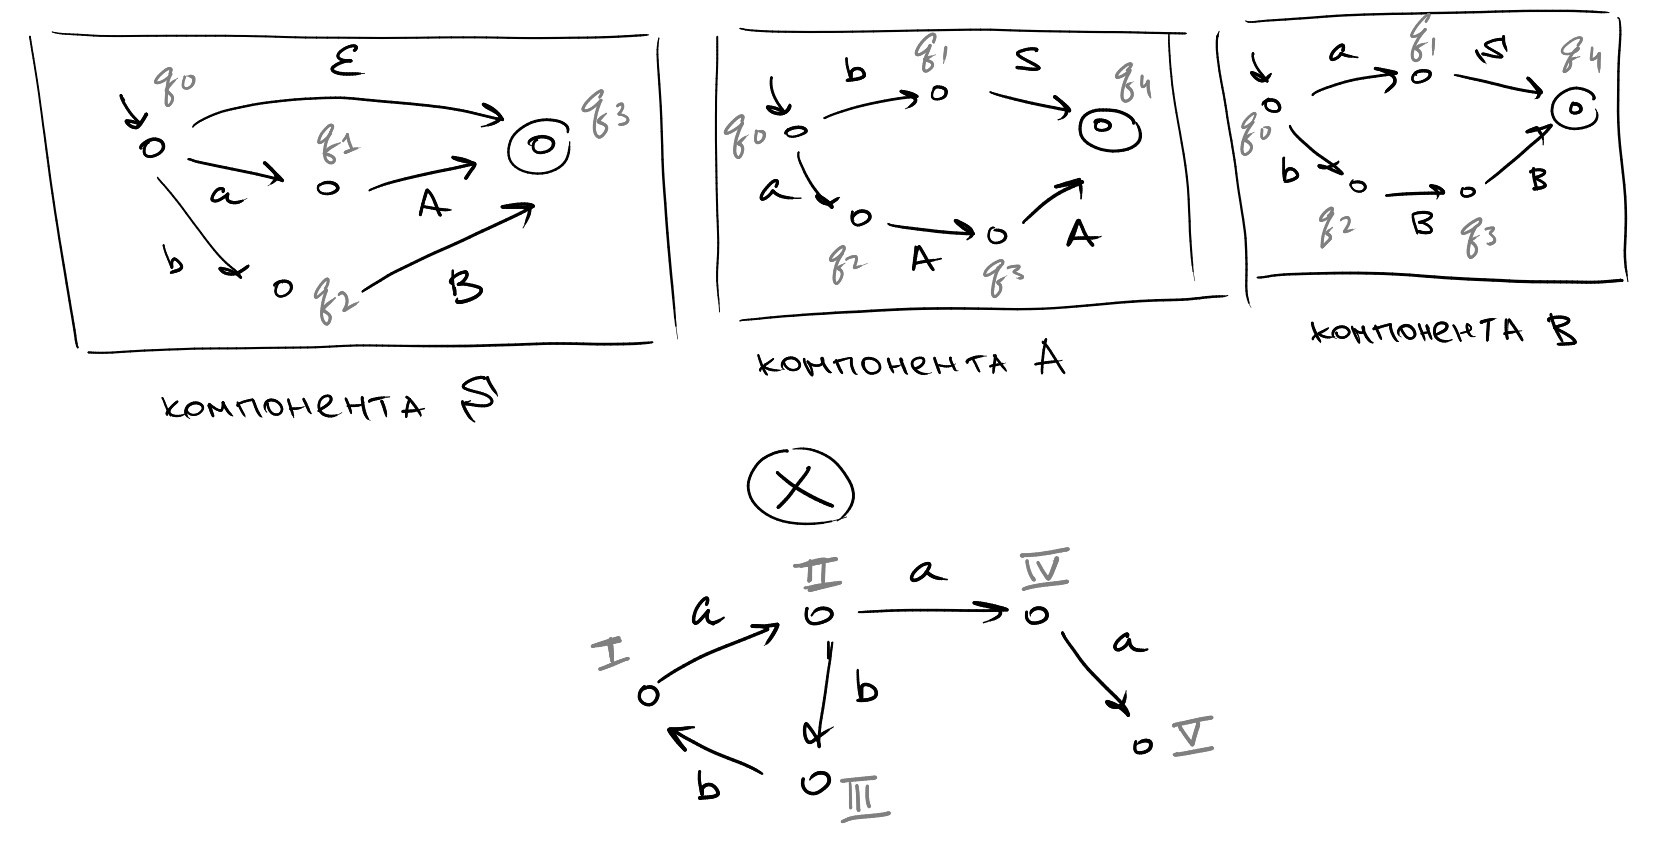
\includegraphics[width=1\linewidth]{img/example_intersection1.png}

        \TODO: дорисовать пример (а потом перерисовать)

    \end{example}

    \TODO: Доказательство корректности сведения (?)


    \TODO: сделать на него ссылки везде (не только на него)

    Все алгоритмы для CFPQ, которые будут описаны в этой работе имеют следующую схему:
    \begin{enumerate}
        \item Построим прямое произведение входной грамматики $\cool{R}$ и входного графа $G$: $\cool{P} = \cool{R} \otimes G$.
        \item \textit{Решим задачу достижимости для полученного РКА $\cool{P}$}
        \item Из вершины $u$ в вершину $v$ входного графа существует путь, выводимой входной грамматикой $\cool{G}$ $\EQ$ в $\cool{P}$ есть путь из стартового состояния $(q_0, u)$ в конечное состояние $(q_f, v)$
    \end{enumerate}

    Рассмотрим внимательнее второй пункт~--- задачу достижимости для РКА. В случае обычного автомата эта задача эквивалентна задаче построения транзитивного замыкания~\cite{Yannakakis1990}. В случае же РКА задача осложняется наличием рекурсивных вызовов, которые разрешаются итеративно. (??)

\subsection{Алгоритм П}

    В листинге~\ref{algo:P} приведён псевдокод Алгоритма П.

    \TODO: что-то написать про епс-переходы

    \begin{algorithm}[H]
        \floatname{algorithm}{Listing}
        \begin{algorithmic}[1]
        \caption{Алгоритм достижимости для РКА}
        \label{algo:P}
        \Function{RSMReachability}{$\cool{R}$}
            \State{$A \gets$ Adjacency matrix for $\cool{R}$}
            \While{$A$ is changing}
                \State{$A' \gets \textit{transitiveClosure}(A)$}
                \Comment{Построение транзитивного замыкания}
                \For{$i \in 1..k$}
                   \For{$u \in En_i$}
                        \For{$v \in Ex_i$}
                            \If{$A'_{u,v} \wedge \overline{A_{u,v}}$}
                                \State{$A' \gets A' \cup getEdges(i, u, v)$}
                                \Comment{Добавление новых рёбер}
                            \EndIf
                        \EndFor
                   \EndFor
                \EndFor
                \State{$A \to A'$}
            \EndWhile
        \State \Return $A$
        \EndFunction
        \end{algorithmic}
    \end{algorithm}

    Работа происходит над матрицей смежности $\cool{R}$~--- изначально туда записываются все ``внутренние'' (нерекурсивные) рёбра. 

    Далее, внешний цикл повторяется, пока матрица смежности $A$ меняется (т.е. пока добавляются новые рёбра). На каждой итерации считается $A'$~--- транзитивное замыкание $A$. После этого находятся все новые пути вида $\langle$стартовое состояние$\rangle$ $\path$ $\langle$конечное состояние$\rangle$~--- те рёбра между стартовой и конечной вершинами компоненты, которых не было в $A$, но которые есть в $A'$~--- и добавляются соответствующие этим путям рёбра: для нового пути $(u \in En_i) \path (v \in Ex_i)$ проводятся все рёбра, соответствующие рекурсивным вызовам $i$-ой компоненты с начальной вершиной $u$ и конечной вершиной $v$.

\subsubsection{Пример}

\TODO

\subsubsection{Время работы}

    Время работы~--- $k \cdot T(n)$, где $k$~--- число итераций внешнего цикла, $T(n)$~--- время работы одной итерации. 

    Оценим $T(n)$. Внутренняя часть цикла состоит из двух частей: нахождения транзитивного замыкания (строка 4) и прохода по матрице для выявления новых рёбер (строки 5-9). 

    Задача поиска транзитивного замыкания эквивалентна задаче перемножения булевых матриц~\cite{Aho1974} и может быть решена сведением к быстрому перемножению (обычных) матриц за $\O(n^\omega)$, где $2 < \omega < 2.273$~\cite{Alman20}.

    Проход по матрице (строки 5-7) работает за $\O(n^2)$, что доминируется временем построения транзитивного замыкания. Добавление новых рёбер (строки 8-9) отработает суммарно за $\O(n^2)$ (т.к. каждое ребро будет добавлено не более одного раза).

    Итого, время работы алгоритма $\O(k \cdot n^{\omega})$.

\subsection{Алгоритм П2}

    Можно заметить, что не очень осмысленно на каждой итерации заново считать транзитивное замыкание, достаточно искать только пути, проходящие через рёбра, добавленные непосредственно на предыдущей итерации. То есть достаточно решать задачу {\bf инкрементального} транзитивного замыкания. 

    В листинге~\ref{algo:P2} приведён псевдокод Алгоритма П2 (основанного на инкрементальном ТЗ)

    \begin{algorithm}[H]
        \floatname{algorithm}{Listing}
        \begin{algorithmic}[1]
        \caption{Алгоритм достижимости для РКА (2)}
        \label{algo:P2}
        \Function{RSMReachability2}{$\cool{R}$}
            \State{$A \gets$ Empty adjacency matrix}
            \State{$Q \gets$ Empty Queue}
            \For{$i \in 1..k$}
                \For{$u \xrightarrow{c} v \in \delta_i$}
                    \State{$Q.Push(\q{u, v, i})$}
                \EndFor
            \EndFor
            \While{$Q$ is not Empty}
                \State{$\q{u, v, i} \gets Q.Pop()$}
                \If{$u \in En_i \wedge v \in En_i$}
                    \Comment{Нашли новый путь}
                    \State{$A \gets A \cup getEdges(i, u, v)$}
                    \State{$Q.PushAll(getEdges(i, u, v))$}
                    \Comment{Добавляем новые рёбра}
                \EndIf
                \For{$x \in Q_i$}
                    \If{$A_{x, u} \wedge \overline{A_{x, v}}$}
                        \For{$y \in Q_i$} 
                            \If{$A_{v, y} \wedge \overline{A_{x, y}}$}
                                \State{$A \gets A \cup \q{x, y}$}
                                \State{$Q.Push(\q{x, y, i})$}
                                \Comment{Обновлем транзитивное замыкание}
                            \EndIf
                        \EndFor
                    \EndIf
                \EndFor
            \EndWhile
        \State \Return $A$
        \EndFunction
        \end{algorithmic}
    \end{algorithm}

    В алгоритме используется (более менее) стандартная реализация инкрементального транзитивного замыкания~\cite{Ibaraki1983}. Для этого в ходе работы алгоритма поддерживается рабочая очередь $Q$ рёбер транзитивного замыкания, которые были найдены, но ещё не обработаны. 

    При обработке очередного \textit{(потому что оно из очереди ахахах)} ребра, ищутся новые пути, которые проходя через него. А именно, пусть было добавлено ребро $u \to v$. Тогда далее перебирается вершина $x$, такая что из неё была достижима вершина $u$ ($x \path u$), но не была достижима вершина $v$ ($x \not\path v$). Из такой вершины $x$ становятся достижимы все вершины $y$, которые были достижимы из $v$ ($v \path y$).

    Также, как и в Алгоритме П, если ребро ТЗ (= путь в графе) соединяет начальную и конечную вершину, в очередь добавляются также все соответствующие ему рекурсивные рёбра.

    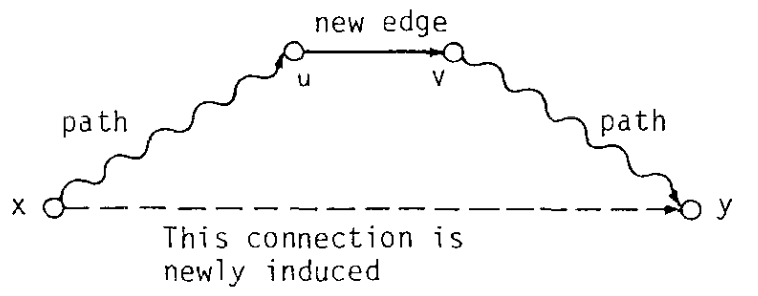
\includegraphics[width=0.75\linewidth]{img/TC_add.png}

    \TODO: норм картинка

\subsubsection{Время работы}

Внешний цикл итерируется по всем рёбрам, так что работает за $\O(m^{*})$. Добавление новых рёбер как и в алгоритме П рассмотрит каждое ребро не более одного раза, так что тоже работает за $O(m^{*})$. Нужно только оценить работу по поддержанию транзитивного замыкания. 

Цикл на строке 12 перебирает все вершины, так что отработает суммарно за $\O(m^{*} n)$. Внутренний цикл (строка 14) тоже перебирает все вершины, но после его выполнения будет добавлено хотя бы одно новое ребро ($x \to v$), так что суммарное время работы этих циклов также можно оценить как $\O(m^{*} n)$.

Итого, суммарное время работы составляет $\O(n m^{*})$, что в плотных графах будет равно $\Theta(n^3)$. 

\begin{note}
Время работы итеративного транзитивного замыкания можно ускорить в $\log n$ раз~\cite{Chaudhuri08}, воспользовавшись методом четырёх русских~\cite{Arlazarov70} (так как работа происходит над булевыми векторами).
\end{note}

\subsection{Выводы и результаты по главе}

\TODO
